\documentclass{article}

\usepackage{fancyhdr}
\usepackage{extramarks}
\usepackage{amsmath}
\usepackage{amsthm}
\usepackage{amsfonts}
\usepackage{tikz}
\usepackage[plain]{algorithm}
\usepackage{algpseudocode}
\usepackage{enumerate}
\usepackage{amssymb}
\usepackage{tikz}
\usepackage{multicol,multirow,array,listings,tabularx,lastpage,textcomp,booktabs}
\usetikzlibrary{automata,positioning,arrows}

%
% Basic Document Settings
%

\topmargin=-0.45in
\evensidemargin=0in
\oddsidemargin=0in
\textwidth=6.5in
\textheight=9.0in
\headsep=0.25in

\linespread{1.1}

\pagestyle{fancy}
\lhead{\hmwkAuthorName}
\chead{\hmwkClass:\ \hmwkTitle}
\rhead{\firstxmark}
\lfoot{\lastxmark}
\cfoot{\thepage}

\renewcommand\headrulewidth{0.4pt}
\renewcommand\footrulewidth{0.4pt}

\setlength\parindent{0pt}
\setlength{\parskip}{5pt}

%
% Create Problem Sections
%

\newcommand{\enterProblemHeader}[1]{
  \nobreak\extramarks{}{Problem \arabic{#1} continued on next page\ldots}\nobreak{}
  \nobreak\extramarks{Problem \arabic{#1} (continued)}{Problem \arabic{#1} continued on next page\ldots}\nobreak{}
}

\newcommand{\exitProblemHeader}[1]{
  \nobreak\extramarks{Problem \arabic{#1} (continued)}{Problem \arabic{#1} continued on next page\ldots}\nobreak{}
  \stepcounter{#1}
  \nobreak\extramarks{Problem \arabic{#1}}{}\nobreak{}
}

\setcounter{secnumdepth}{0}
\newcounter{partCounter}
\newcounter{homeworkProblemCounter}
\setcounter{homeworkProblemCounter}{1}
\nobreak\extramarks{Problem \arabic{homeworkProblemCounter}}{}\nobreak{}

%
% Homework Problem Environment
%
% This environment takes an optional argument. When given, it will adjust the
% problem counter. This is useful for when the problems given for your
% assignment aren't sequential. See the last 3 problems of this template for an
% example.
%
\newenvironment{homeworkProblem}[1][-1]{
  \ifnum#1>0
      \setcounter{homeworkProblemCounter}{#1}
  \fi
  \section{Problem \arabic{homeworkProblemCounter}}
  \setcounter{partCounter}{1}
  \enterProblemHeader{homeworkProblemCounter}
}{
  \exitProblemHeader{homeworkProblemCounter}
}

\newcommand\abs[1]{\lvert~#1~\rvert}
\newcommand{\st}{\mid}

\newcommand{\cmark}{\ding{51}}
\newcommand{\xmark}{\ding{55}}
 
\newcommand{\SUBSTRING}{\textsc{Substring}}
\newcommand{\REP}{\textsc{Rep}}
\newcommand{\blank}{\scalebox{1.5}{\textvisiblespace}}

%
% Homework Details
%   - Title
%   - Due date
%   - Class
%   - Section/Time
%   - Instructor
%   - Author
%

\newcommand{\hmwkTitle}{Homework\ \#2}
\newcommand{\hmwkDueDate}{Feb 1, 2023}
\newcommand{\hmwkClass}{CSE 105}
\newcommand{\hmwkClassInstructor}{Professor Minnes}
\newcommand{\hmwkAuthorName}{\textbf{Ray Tsai}}
\newcommand{\hmwkPID}{A16848188}

\newcommand{\gradeCorrect}{({\it Graded for correctness}) }
\newcommand{\gradeCorrectFirst}{\gradeCorrect\footnote{This means your solution will be evaluated
not only on the correctness of your answers, but on your ability to present your ideas clearly and
logically. You should explain how you arrived at your conclusions, using mathematically sound
reasoning. Whether you use formal proof techniques or write a more informal argument for why
something is true, your answers should always be well-supported. Your goal should be to convince the
reader that your results and methods are sound.} } 
\newcommand{\gradeComplete}{({\it Graded for completeness}) } 
\newcommand{\gradeCompleteFirst}{\gradeComplete\footnote{This means you will get full credit so long
as your submission demonstrates honest effort to answer the question. You will not be penalized for
incorrect answers. To demonstrate your honest effort in answering the question, we expect you to
include your attempt to answer *each* part of the question. If you get stuck with your attempt, you
can still demonstrate your effort by explaining where you got stuck and what you did to try to get
unstuck.} }

%
% Title Page
%

\title{
    \vspace{2in}
    \textmd{\textbf{\hmwkClass:\ \hmwkTitle}}\\
    \normalsize\vspace{0.1in}\small{Due\ on\ \hmwkDueDate\ at 23:59pm}\\
    \vspace{0.1in}\large{\textit{\hmwkClassInstructor}} \\
    \vspace{3in}
}

\author{
  \hmwkAuthorName \\
  \vspace{0.1in}\small\hmwkPID
}
\date{}

\renewcommand{\part}[1]{\textbf{\large Part \Alph{partCounter}}\stepcounter{partCounter}\\}

%
% Various Helper Commands
%

% Useful for algorithms
\newcommand{\alg}[1]{\textsc{\bfseries \footnotesize #1}}

% For derivatives
\newcommand{\deriv}[1]{\frac{\mathrm{d}}{\mathrm{d}x} (#1)}

% For partial derivatives
\newcommand{\pderiv}[2]{\frac{\partial}{\partial #1} (#2)}

% Integral dx
\newcommand{\dx}{\mathrm{d}x}

% Probability commands: Expectation, Variance, Covariance, Bias
\newcommand{\Var}{\mathrm{Var}}
\newcommand{\Cov}{\mathrm{Cov}}
\newcommand{\Bias}{\mathrm{Bias}}
\newcommand*{\Z}{\mathbb{Z}}
\newcommand*{\Q}{\mathbb{Q}}
\newcommand*{\R}{\mathbb{R}}
\newcommand*{\C}{\mathbb{C}}
\newcommand*{\N}{\mathbb{N}}
\newcommand*{\prob}{\mathds{P}}
\newcommand*{\E}{\mathds{E}}

\begin{document}

\maketitle

\pagebreak

\begin{homeworkProblem}
  Integers can be represented using base $b$ expansions, for a convenient choice of base $b$: for
  $b$ an integer greater than $1$ and $n$ a positive integer, the {\bf base $b$ expansion of $n$} is
  defined to be
  \[
    (a_{k-1} \cdots a_1 a_0)_b
  \]
  where $k$ is a positive integer, $a_0, a_1, \ldots, a_{k-1}$ are nonnegative integers less than
  $b$, $a_{k-1} \neq  0$, and
  \[
    n = \sum_{i=0}^{k-1} a_{i} b^{i}
  \]
  
  Notice: {\it The base $b$ expansion of a positive integer $n$ is a string over the alphabet $\{x
  \in \mathbb{Z} \st 0 \leq x < b\}$ whose leftmost character is nonzero.}
  
  An important property of base $b$ expansions of integers is that, for each integer $b$ greater
  than $1$, each positive integer $n = (a_{k-1} \cdots a_1 a_0)_b$, and each nonnegative integer $a$
  less than $b$, 
  \[
    bn + a = (a_{k-1} \cdots a_1 a_0a)_b
  \]
  In other words, shifting the base $b$ expansion to the left results in multiplying the integer
  value by the base. In this question we'll explore building deterministic finite automata that
  recognize languages that correspond to useful sets of integers.
  
  \begin{enumerate}[(a)]
  \item Design a DFA that recognizes the set of binary (base $2$) expansions of positive integers
  that are powers of $2$. A complete solution will include the state diagram of your DFA and a brief
  justification of your construction by explaining the role each state plays in the machine, as well
  as a brief justification about how the strings accepted and rejected by the machine connect to the
  specified language.

  \begin{proof}[Solution]
    Consider the following state diagram of a DFA:
    \begin{center}
      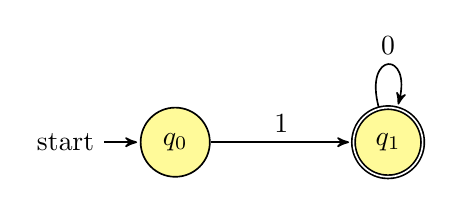
\begin{tikzpicture}[->,>=stealth',shorten >=1pt, auto, node distance=2cm, semithick]
      \tikzstyle{every state}=[text=black, fill=yellow!40]
    
      \node[initial, state] (q0)          {$q_0$};
      \node[state, accepting] (q1) [right of=q0, xshift=20pt] {$q_1$};
    
      \path (q0) edge [left=20, above] node {$1$} (q1)
            (q1) edge [loop above] node {$0$} (q1)
      ;
      \end{tikzpicture}
    \end{center}
    The base 2 representations of all powers of two only have the first digit as 1 and 0 for the
    rest, $10^*$ in regular expression, and this the exact language that the above DFA
    accepts.
  \end{proof}

  \item Consider arbitrary positive integer $m$. Design a DFA that recognizes the set of binary
  (base $2$) expansions of positive integers that are multiples of $m$. A complete solution will
  include the formal definition of your DFA (paramterized by $m$) and a brief justification of your
  construction by explaining the role each state plays in the machine, as well as a brief
  justification about how the strings accepted and rejected by the machine connect to the specified
  language.

  \begin{proof}[Solution]
    Consider a DFA $(\Z_m, \Sigma = \{0, 1\}, \delta, [0], \{[0]\})$, where the state $[i]$
    represents the $i$-th equivalence class in $\Z_m$ and $\delta: \Z_m \times \Sigma \rightarrow
    \Z_m$ is the transition funtion that maps $([i], \sigma)$ to $[2i + \sigma]$. The states of the
    DFA records the current remainder of the binary string read. Since the current remainder needs
    to be multiplied by 2 every times we read a new digit, $\delta$ updates the current remainder
    and add the value of the new digit accordingly. Thus, a string is accepted if and only if the
    remainder is 0 after the string is fully processed.
  \end{proof}

  \item Choose a positive integer $m_{0}$ between $4$ and $8$ (inclusive) and draw the state diagram
  of a DFA recognizing the language over $\{0,1,2\}$ $$\{ w \in \{0,1,2\}^* \mid w \text{ is a base
  $3$ expansion of a positive integer that is a multiple of $m_0$}\}$$ A complete solution will
  include the state diagram of your DFA and a brief justification of your construction by explaining
  the role each state plays in the machine, as well as a brief justification about how the strings
  accepted and rejected by the machine connect to the specified language.

  \begin{proof}[Solution]
    Let $m_0 = 4$ and consider the following state diagram of a DFA:
    \begin{center}
      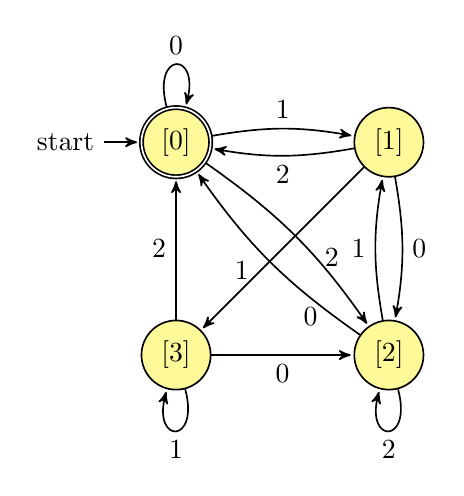
\begin{tikzpicture}[->,>=stealth',shorten >=1pt, auto, node distance=2cm, semithick]
      \tikzstyle{every state}=[text=black, fill=yellow!40]
    
      \node[initial, state, accepting] (q0) {$[0]$};
      \node[state] (q1) [right of=q0, xshift=20] {$[1]$};
      \node[state] (q2) [below of=q1, yshift=-20] {$[2]$};
      \node[state] (q3) [below of=q0, yshift=-20] {$[3]$};
    
      \path (q0)  edge [loop above] node {$0$} (q0)
                  edge [bend left=10, above] node {$1$} (q1)
                  edge [bend left=10, above, near end] node {$2$} (q2)
            (q1)  edge [bend left=10, right] node {$0$} (q2)
                  edge [above, near end] node {$1$} (q3)
                  edge [bend left=10, below] node {$2$} (q0)
            (q2)  edge [bend left=10, below, near start] node {$0$} (q0)
                  edge [bend left=10, left] node {$1$} (q1)
                  edge [loop below] node {$2$} (q2)
            (q3)  edge [below] node {$0$} (q2)
                  edge [loop below] node {$1$} (q3)
                  edge [left] node {$2$} (q0)
      ;
      \end{tikzpicture}
    \end{center}
    Each state represents an equivalence class in $\Z_4$, and they all together play the role of
    recording the current remainder of the string, upon dividing by $4$. Note that upon reading a
    new digit $\sigma$, state $[i]$ would be mapped to state $[2i + \sigma]$, and a string would get
    accepted if and only if it ends at state $[0]$ after being copletely processed. In other words,
    a string would get accepted if and only if it ends it is a multiple of $4$.
  \end{proof}
  \end{enumerate}
\end{homeworkProblem}

\newpage

\begin{homeworkProblem}
  For any language $L \subseteq \Sigma^*$, recall that we define its \emph{complement} as
  $$\overline{L} := \Sigma^* - L = \{w \in \Sigma^* \mid w \notin L\}$$ That is, the complement of
  $L$ contains all and only those strings which are not in $L$. Our notation for regular expressions
  does not include the complement symbol. However, it turns out that the complement of a language
  described by a regular expression is guaranteed to also be describable by a (different) regular
  expression. For example, over the alphabet $\Sigma = \{0,1\}$, the complement of the language
  described by the regular expression $\Sigma^* 0$ is described by the regular expression
  $\varepsilon \cup \Sigma^*1$ because any string that does not end in $0$ must either be the empty
  string or end in $1$.

  For each of the regular expressions $R$ over the alphabet $\Sigma = \{a,b\}$ below, write the
  regular expression for~$\overline{L(R)}$. Your regular expressions may use the symbols
  $\varnothing$, $\varepsilon$, $a$, $b$, and the following operations to combine them: union,
  concatenation, and Kleene star.

  Briefly justify why your solution for each part works by giving plain English descriptions of the
  language described by the regular expression and of its complement and connecting them to the
  regular expression via relevant definitions. An English description that is more detailed than
  simply negating the description in the original language will likely be helpful in the
  justification.

  Alternatively, you can justify your solution by first designing a DFA that recognizes $L(R)$,
  using the construction from class and the book to modify this DFA to get a new DFA that
  recognizes~$\overline{L(R)}$, and then applying the constructions from class and the book to
  convert this new DFA to a regular expression.

  For each part of the question, clearly state which approach you're taking and include enough
  intermediate steps to illustrate your work.

\begin{enumerate}[(a)]
    \item $a^*b^*$
    \begin{proof}[Solution]
      Consider $(a \cup b)^*ba(a \cup b)^*$. Since $L(a^*b^*)$ is the set of strings that has no $b$
      preceding $a$, $\overline{L(a^*b^*)}$ is the set of strings that has at least a $b$ preceding
      an $a$, which much contain at least a substring $ba$. Thus, $(a \cup b)^*ba(a \cup b)^*$
      describes the set.
    \end{proof}
    \item $(a \cup b) a b^*$
    \begin{proof}
      Consider a disturbingly straight forward example $\epsilon \cup (a \cup b) \cup (a \cup b)b(a
      \cup b)^* \cup (a \cup b)(a \cup b)^+a(a \cup b)^*$. Since the negation of $(a \cup b) a b^*$
      is a string that has length less than 2 or doesn't have $a$ as its second character or
      contains at least an $a$ after the second character, we take the union of all conditions and
      obtain the resulting regular expression.
    \end{proof}
\end{enumerate}
\end{homeworkProblem}

\newpage

\begin{homeworkProblem}
  In this question, you'll practice working with formal general constructions for DFAs and
  translating between state diagrams and formal definitions. Consider the following general
  construction: Let $N_1 = (Q, \Sigma, \delta_1, q_1, F_1)$ be a NFA and assume that $q_0 \notin Q$.
  Define the new NFA $N_2 = (Q \cup \{q_0\}, \Sigma, \delta_2, q_0, \{q_1\})$ where 
  $$\delta_2: (Q \cup \{q_0\}) \times \Sigma_\varepsilon \to (Q \cup \{q_0\})$$ is defined by
  \[
    \delta_2 (q,a) = \begin{cases}
      \{ q' \in Q \mid q \in \delta_1(q',a)\} &\text{if $q \in Q$, $a \in \Sigma_{\varepsilon}$} \\
      F_1 &\text{if $q =q_0$, $a = \varepsilon$}\\
      \emptyset &\text{if $q = q_0$, $a \in \Sigma$}
    \end{cases}
  \]

\begin{enumerate}[(a)]
  \item Illustrate this construction by defining a specific example NFA $N$ and applying the
  construction above to create a new NFA. Your example NFA should
  \begin{itemize}
      \item Have exactly three states (all reachable from the start state),
      \item Have at least one spontaneous move (arrow labelled $\varepsilon$),
      \item Accept at least one string and reject at least one string, and
      \item Not have any states labelled $q_0$.
  \end{itemize}
  Apply the construction above to create the new NFA. A complete submission will include the state
  diagram of your example NFA $N$ and the state diagram of the NFA resulting from this construction.
  \begin{proof}[Solution]
    Consider the following state diagram of NFA $N$:
    \begin{center}
      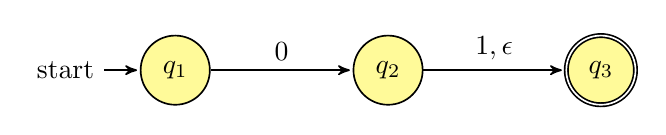
\begin{tikzpicture}[->,>=stealth',shorten >=1pt, auto, node distance=2cm, semithick]
      \tikzstyle{every state}=[text=black, fill=yellow!40]
    
      \node[initial, state] (q1)          {$q_1$};
      \node[state] (q2) [right of=q1, xshift=20pt] {$q_2$};
      \node[state, accepting] (q3) [right of=q2, xshift=20pt] {$q_3$};
    
      \path (q1) edge [left=20, above] node {$0$} (q2)
            (q2) edge [left=20, above] node {$1, \epsilon$} (q3)
      ;
      \end{tikzpicture}
    \end{center}
    Note that $N$ accepts $0$ and rejects $1$. The state diagram of the NFA resulting from this
    construction upon $N$ is:
    \begin{center}
      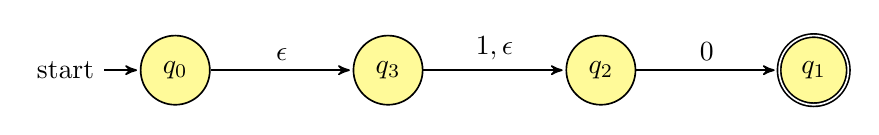
\begin{tikzpicture}[->,>=stealth',shorten >=1pt, auto, node distance=2cm, semithick]
      \tikzstyle{every state}=[text=black, fill=yellow!40]
    
      \node[initial, state] (q0)      {$q_0$};
      \node[state] (q3) [right of=q0, xshift=20pt] {$q_3$};
      \node[state] (q2) [right of=q3, xshift=20pt] {$q_2$};
      \node[state, accepting] (q1) [right of=q2, xshift=20pt] {$q_1$};
    
      \path (q0) edge [left=20, above] node {$\epsilon$} (q3)
            (q2) edge [left=20, above] node {$0$} (q1)
            (q3) edge [left=20, above] node {$1, \epsilon$} (q2)
      ;
      \end{tikzpicture}
    \end{center}
  \end{proof}

  \newpage

  \item Use Theorem 1.39 on page 55 of the book (see also page 7 in Week 3 notes) to construct a DFA
  equivalent to your example NFA $N$ from part (a). A complete submission will include the state
  diagram of your example NFA $N$ and the state diagram of the DFA resulting from this construction,
  with the correct state labels for this DFA. You may prune the DFA so that only the
  ``macro-states'' reachable from the start state are included.
  \begin{proof}
    The DFA equivalent of $N$ from part (a) is
    \begin{center}
      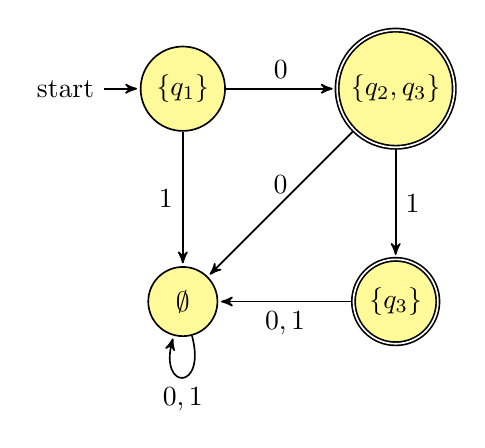
\begin{tikzpicture}[->,>=stealth',shorten >=1pt, auto, node distance=2cm, semithick]
      \tikzstyle{every state}=[text=black, fill=yellow!40]
    
      \node[initial, state] (q1)          {$\{q_1\}$};
      \node[state, accepting] (q23) [right of=q1, xshift=20pt] {$\{q_2, q_3\}$};
      \node[state, accepting] (q3) [below of=q23, yshift=-20pt] {$\{q_3\}$};
      \node[state] (null) [below of=q1, yshift=-20pt] {$\emptyset$};
    
      \path (q1) edge [left=20, above] node {$0$} (q23)
            (q1) edge [left=20, left] node {$1$} (null)
            (q23) edge [left=20, right] node {$1$} (q3)
            (q23) edge [left=20, above] node {$0$} (null)
            (q3) edge [left=20, below] node {$0, 1$} (null)
            (null) edge [loop below] node {$0, 1$} (null)
      ;
      \end{tikzpicture}
    \end{center}
  \end{proof}
  \item Explain the relationship between $N_1$ and $N_2$ in the general construction. Give an
  example string that is accepted by your example NFA $N$ and is rejected by the NFA that results
  from applying the general construction that illustrates this relationship, or explain why there is
  no such example string.
  \begin{proof}
    $N_2$ accepts the reverse of the strings accepted by $N_1$. Formally, $L(N_2) = \{w \in
    \Sigma^* \mid w^{\mathcal{R}} \in L(N_1)\}$. For example, $01$ is accepted by $N$ but not by the
    NFA that results from applying the general construction.
  \end{proof}
\end{enumerate}
\end{homeworkProblem}

\newpage

\begin{homeworkProblem}
  \begin{enumerate}[(a)]
    \item Give an example of a language over the alphabet $\{0,1\}$ that has cardinality $3$ and for
    which $5$ is a pumping length and $4$ is not a pumping length.  A complete solution will give a
    clear and precise description of the language, a justification for why $5$ is a pumping length,
    and a justification for why $4$ is not a pumping length. Is this language regular?
    \begin{proof}[Solution]
      Consider the set $L = \{0, 00, 0000\}$. Since $L$ doesn't contain any string of length at
      least 5, $5$ is a valid pumping length. However, $4$ is not a valid pumping length, as $0000$
      cannot be pumped. Since $L$ is of a finite cardinality, there exists a DFA that accepts $L$,
      and thus $L$ is regular.
    \end{proof}
    \item Consider the following attempted ``proof" that the set 
    $$X = \{ uw \mid \text{$u$ and $w$ are strings over $\{0,1\}$ and have the same length} \}$$ is
    nonregular.
    \begin{quote}
    ``Proof" that $X_1$ is not regular using the Pumping Lemma: Let $p$ be an arbitrary positive
    integer. We will show that $p$ is not a pumping length for $X_1$. 
    
    Choose $s$ to be the string $1^p 0^p$, which is in $X_1$ because we can choose $u = 1^p$ and $w
    = 0^p$ which each have length $p$. Since $s$ is in $X_1$ and has length greater than or equal to
    $p$, if $p$ were to be a pumping length for $X_1$, $s$ ought to be pump'able. That is, there
    should be a way of dividing $s$ into parts $x,y,z$ where $s=xyz$, $|y| >0$, $|xy| \leq p$, and
    for each $i \geq 0$, $xy^iz \in X_1$. Suppose $x,y,z$ are such that $s = xyz$, $|y| > 0$ and
    $|xy| \leq p$. Since the first $p$ letters of $s$ are all $1$ and $|xy| \leq p$, we know that
    $x$ and $y$ are made up of all $1$s.  If we let $i=2$, we get a string $xy^iz$ that is not in
    $X_1$ because repeating $y$ twice adds $1$s to $u$ but not to $w$, and strings in $X_1$ are
    required to have $u$ and $w$ be the same length. Thus, $s$ is not pumpable (even though it
    should have been if $p$ were to be a pumping length) and so $p$ is not a pumping length for
    $X_1$.  Since $p$ was arbitrary, we have demonstrated that $X_1$ has no pumping length.  By the
    Pumping Lemma, this implies that $X_1$ is nonregular.
    \end{quote}
    Find the (first and/or most significant) logical error in the ``proof" and describe why it's
    wrong. Then, either prove that the set is actually regular (by finding a regular expression that
    describes it or a DFA/NFA that recognizes it, and justifying why) {\bf or} fix the proof so that
    it is logically sound.

    \begin{proof}[Solution]
      The statement ``if we let $i=2$, we get a string $xy^iz$ that is not in $X_1$ because
      repeating $y$ twice adds $1$s to $u$ but not to $w$, and strings in $X_1$ are required to have
      $u$ and $w$ be the same length,'' is incorrect, as $u$ and $w$ are not fixed. Since the
      modified string remains to have even length, we may pick $u$ to be the first half of the new
      string and $w$ to be the second half. Since $u, w \in \{0, 1\}^*$ and of the same length, the
      new string is in $X$.

      To show that $X$ is regular, consider the regular expression $((0 \cup 1)^2)^*$. Since this
      regular expression describes all strings $s$ of even length, we may choose $u$ to be the first
      half of the string and $w$ to be the second half. Since $u, w$ are both strings over $\{0,
      1\}$ and are of the same length, $s \in X$. Conversely, suppose that $s$ not encompassed by
      the regular expression. Then, $s$ is of odd length, so there does not exists $u, w$ that are
      of the same length, and thus $s \notin X$.
    \end{proof}
    
    \newpage
    
    \item In class and in the reading so far, we've seen the following examples of nonregular sets:
    \begin{multicols}{3}
    \begin{center}
    $\{ 0^n 1^n ~|~ n \geq 0 \}$
    $$\{ 0^n 1^n ~|~ n \geq 2 \}$$
    $$\{ 0^n 1^m ~|~  0 \leq n \leq m \}$$
    $$\{ 0^n 1^m ~|~ 0 \leq m \leq n \}$$
    $$\{ 0^i 1^{2i} ~|~ 0 \leq i \}$$
    $$\{ 0^i 1^{i+1} ~|~ 0 \leq i \}$$
    $$\{ 0^n 1^m 0^n ~|~n,m \geq 0\}$$
    $$\{ w \in \{0,1\}^* ~|~w = w^R\}$$
    $$\{ w w^R ~|~ w \in \{0,1\}^*\}$$
    \end{center}
    \end{multicols}
    Modify one of these sets in some way and use the Pumping Lemma to prove that the resulting set
    is still nonregular.
    \begin{proof}
      Consider $L = \{ 1^n 0^n ~|~ n \geq 0 \}$. Suppose for the sake of contradiction that $L$ is
      regular. Let $p$ be the pumping length given by the pumping lemma. Consider $s = 1^p0^p$.
      Since $|s| \geq p$, $s$ is pumpable. By the pumping lemma, we may split $s$ into three parts
      $xyz$, where $|xy| \leq p$. Since the first $p$ characters are all $1$'s, $y$ must consist of
      all $1$'s. However, if $i = 2$, we add positive numbers of $1$ into the string but no 0, so
      the numbers of $1$ and 0 in the string are not equal, contradiction. Therefore, $L$ is
      non-regular.
    \end{proof}
    \end{enumerate}
\end{homeworkProblem}

\newpage

\begin{homeworkProblem}
  In Week 2's review quiz, we saw the definition that a set $X$ is said to be {\bf closed under an
  operation} if, for any elements in $X$, applying to them gives an element in $X$. For example, the
  set of integers is closed under multiplication because if we take any two integers, their product
  is also an integer.

  Prove or disprove each closure claim statement below about the class of regular languages and the
  class of nonregular languages. Your arguments may refer to theorems proved in the textbook and
  class, and if they do, should include specific page numbers and references (i.e.\ write out the
  claim that was proved in the book and/or class).

  Recall the definitions we have: 

  For languages $L_1, L_2$ over the alphabet $\Sigma_1 = \{0,1\}$, we have the associated sets of
  strings
  \[
    SUBSTRING(L_1) = \{ w \in \Sigma_1^* ~|~ \text{there exist } a,b \in \Sigma_1^* \text{ such that } awb \in L_1\}
  \]
  and 
  \[
    L_1 \circ L_2 = \{ w \in \Sigma_1^* ~|~ w = uv \text{ for some strings } u \in L_1 \text{ and } v \in L_2 \}
  \]
  \begin{enumerate}

    \item The set of regular languages over $\{0,1\}$ is closed under set-wise concatenation.
    \begin{proof}
      Theorem 1.47 on page 60 of the textbook claims that ``the class of regular languages is close
      under the concatenation operation,'' and thus the result follows.
    \end{proof}

    \item The set of nonregular languages over $\{0,1\}$ is closed under set-wise concatenation.
    \begin{proof}
      This is false. Consider a nonregular language $L$ and its complement $L^c$. Since $L \cup L^c
      = \{0, 1\}^*$ but $\{0, 1\}^*$ is regular, nonregular languages are not closed under set-wise
      concatenation.
    \end{proof}
  
    \item The set of regular languages over $\{0,1\}$ is closed under the $SUBSTRING$ operation.
    \begin{proof}
      Let $N = (Q, \Sigma_1, \delta, q_1, F)$ recognize $L$. 
      
      Construct $N' = (Q', \Sigma_1, \delta', q_0, F')$ to recognize $SUBSTRING(L)$. 

      \begin{enumerate}[i.]
        \item $Q' = Q \cup \{q_0\}$
        \item $F' = \{q \in Q \mid q \in \delta(s), \forall s \in SUBSTRING(L)\}$
        \item Define $\delta'$ so that for any $q \in Q'$ and $a \in \Sigma_{\epsilon}$,
        \[
          \delta' = \begin{cases}
            \delta(q, a), & q \in Q \\
            F', & q = q_0, a = \epsilon \\
            \emptyset, & q = q_0, a \neq \epsilon.
          \end{cases}
        \]
      \end{enumerate}
    \end{proof}

    \item The set of nonregular languages over $\{0,1\}$ is closed under the $SUBSTRING$ operation.
      \begin{proof}
        This is false. Consider $L = \{0^n1^n \mid n \in \N\}$. $L$ is non-regular, shown as example
       1.73 on page 80 of hte textbook. Since $SUBSTRING(L)$ is simply the set of strings where none
       of them have 1 proceding 0, it can be described as $0^*1^*$ in terms of regular expression,
       and thus $SUBSTRING(L)$ is regular.
      \end{proof}
  \end{enumerate}
\end{homeworkProblem}
\end{document}